\section{RELATED WORK}
\label{sec:related_work}


Gesture generation, like other machine learning tasks, has been explored using both traditional rule-based methods and modern data-driven approaches. We first examine the fundamental characteristics of gestures (\autoref{sec:relationspeechandgesture}) as a basis for modeling their relationship with text and speech. \autoref{fig:CommonStage} illustrates the common processing stages shared across various gesture generation techniques.


\subsection{Gesture Characteristics}
\label{sec:relationspeechandgesture}

According to linguistics, gestures can be categorized into six main groups: adaptors, emblems, deictics, iconics, metaphorics, and beats \cite{ekman1969repertoire}, \cite{sebeok2011advances}. Among them, beat gestures do not carry direct semantic meaning but play an important role in synchronizing rhythm between speech and gesture \cite{kipp2005gesture}, \cite{sebeok2011advances}. However, the rhythm between speech and beat gestures is not fully synchronized, making the temporal alignment between them complex to model \cite{mcclave1994gestural}, \cite{bhattacharya2021speech2affectivegestures}, \cite{kucherenko2020gesticulator}, \cite{yoon2020speech}.

Gestures interact with various levels of information in speech \cite{sebeok2011advances}. For instance, emblematic gestures like a thumbs-up are usually linked to high-level semantic content (e.g., “good” or “excellent”), while beat gestures often accompany low-level prosodic features such as emphasis. Previous studies typically extract features from the final layer of the speech encoder to synthesize gestures \cite{alexanderson2020style}, \cite{bhattacharya2021speech2affectivegestures}, \cite{kucherenko2021large}, \cite{qian2021speech}, \cite{yoon2022genea}. However, this approach may blend information from different levels, making it hard to disentangle rhythm and semantics.

As shown in linguistic studies \cite{kipp2005gesture}, \cite{neff2008gesture}, \cite{webb1997linguistic}, gestures in daily communication can be decomposed into a limited number of semantic units with various motion variations. Based on this assumption, speech features are divided into two types: high-level features representing semantic units and low-level features capturing motion variations. Their relationships are learned across different layers of the speech encoder. Experiments demonstrate that this mechanism can effectively disentangle features at different levels and generate gestures that are both semantically and stylistically appropriate.





\subsection{Overview of Gesture Generation Methods}
\label{sec:relatedwork}

\subsubsection{Rule-Based Methods}

These methods rely on clearly defined rules, which are manually crafted to determine how the system processes inputs to produce outputs.

\textbf{Methods}: Representative rule-based methods include the \textit{Robot behavior toolkit} \cite{huang2012robot} and \textit{Animated conversation} \cite{cassell1994animated}. These approaches typically map speech to gesture units using handcrafted rules. Rule-based systems allow for straightforward control over model outputs and provide good interpretability.  
However, the cost of manually designing these rules is prohibitive for complex applications requiring the processing of large-scale data.

\subsubsection{Statistical Methods}

These methods rely on data analysis, learning patterns from datasets, and using probabilistic models or mathematical functions for prediction. The approach involves optimizing model parameters to fit the data.


\textbf{Methods}: Like rule-based methods, data-driven methods also map speech features to corresponding gestures. However, instead of manual rules, they employ automatic learning based on statistical data analysis.

Representative statistical approaches include \textit{Gesture controllers} \cite{levine2010gesture}, \textit{Statistics-based} \cite{yang2020statistics}, which use probabilistic distributions to find similarities between speech and gesture features. \textit{Gesture modeling} \cite{neff2008gesture} constructs probabilistic models to learn individual speaker styles.

\subsubsection{Deep Learning Methods}

These methods utilize multi-layer perceptrons (MLPs) to automatically extract features from raw data and learn complex data representations through parameter optimization.

%\begin{figure}[b]
%	\centering
%	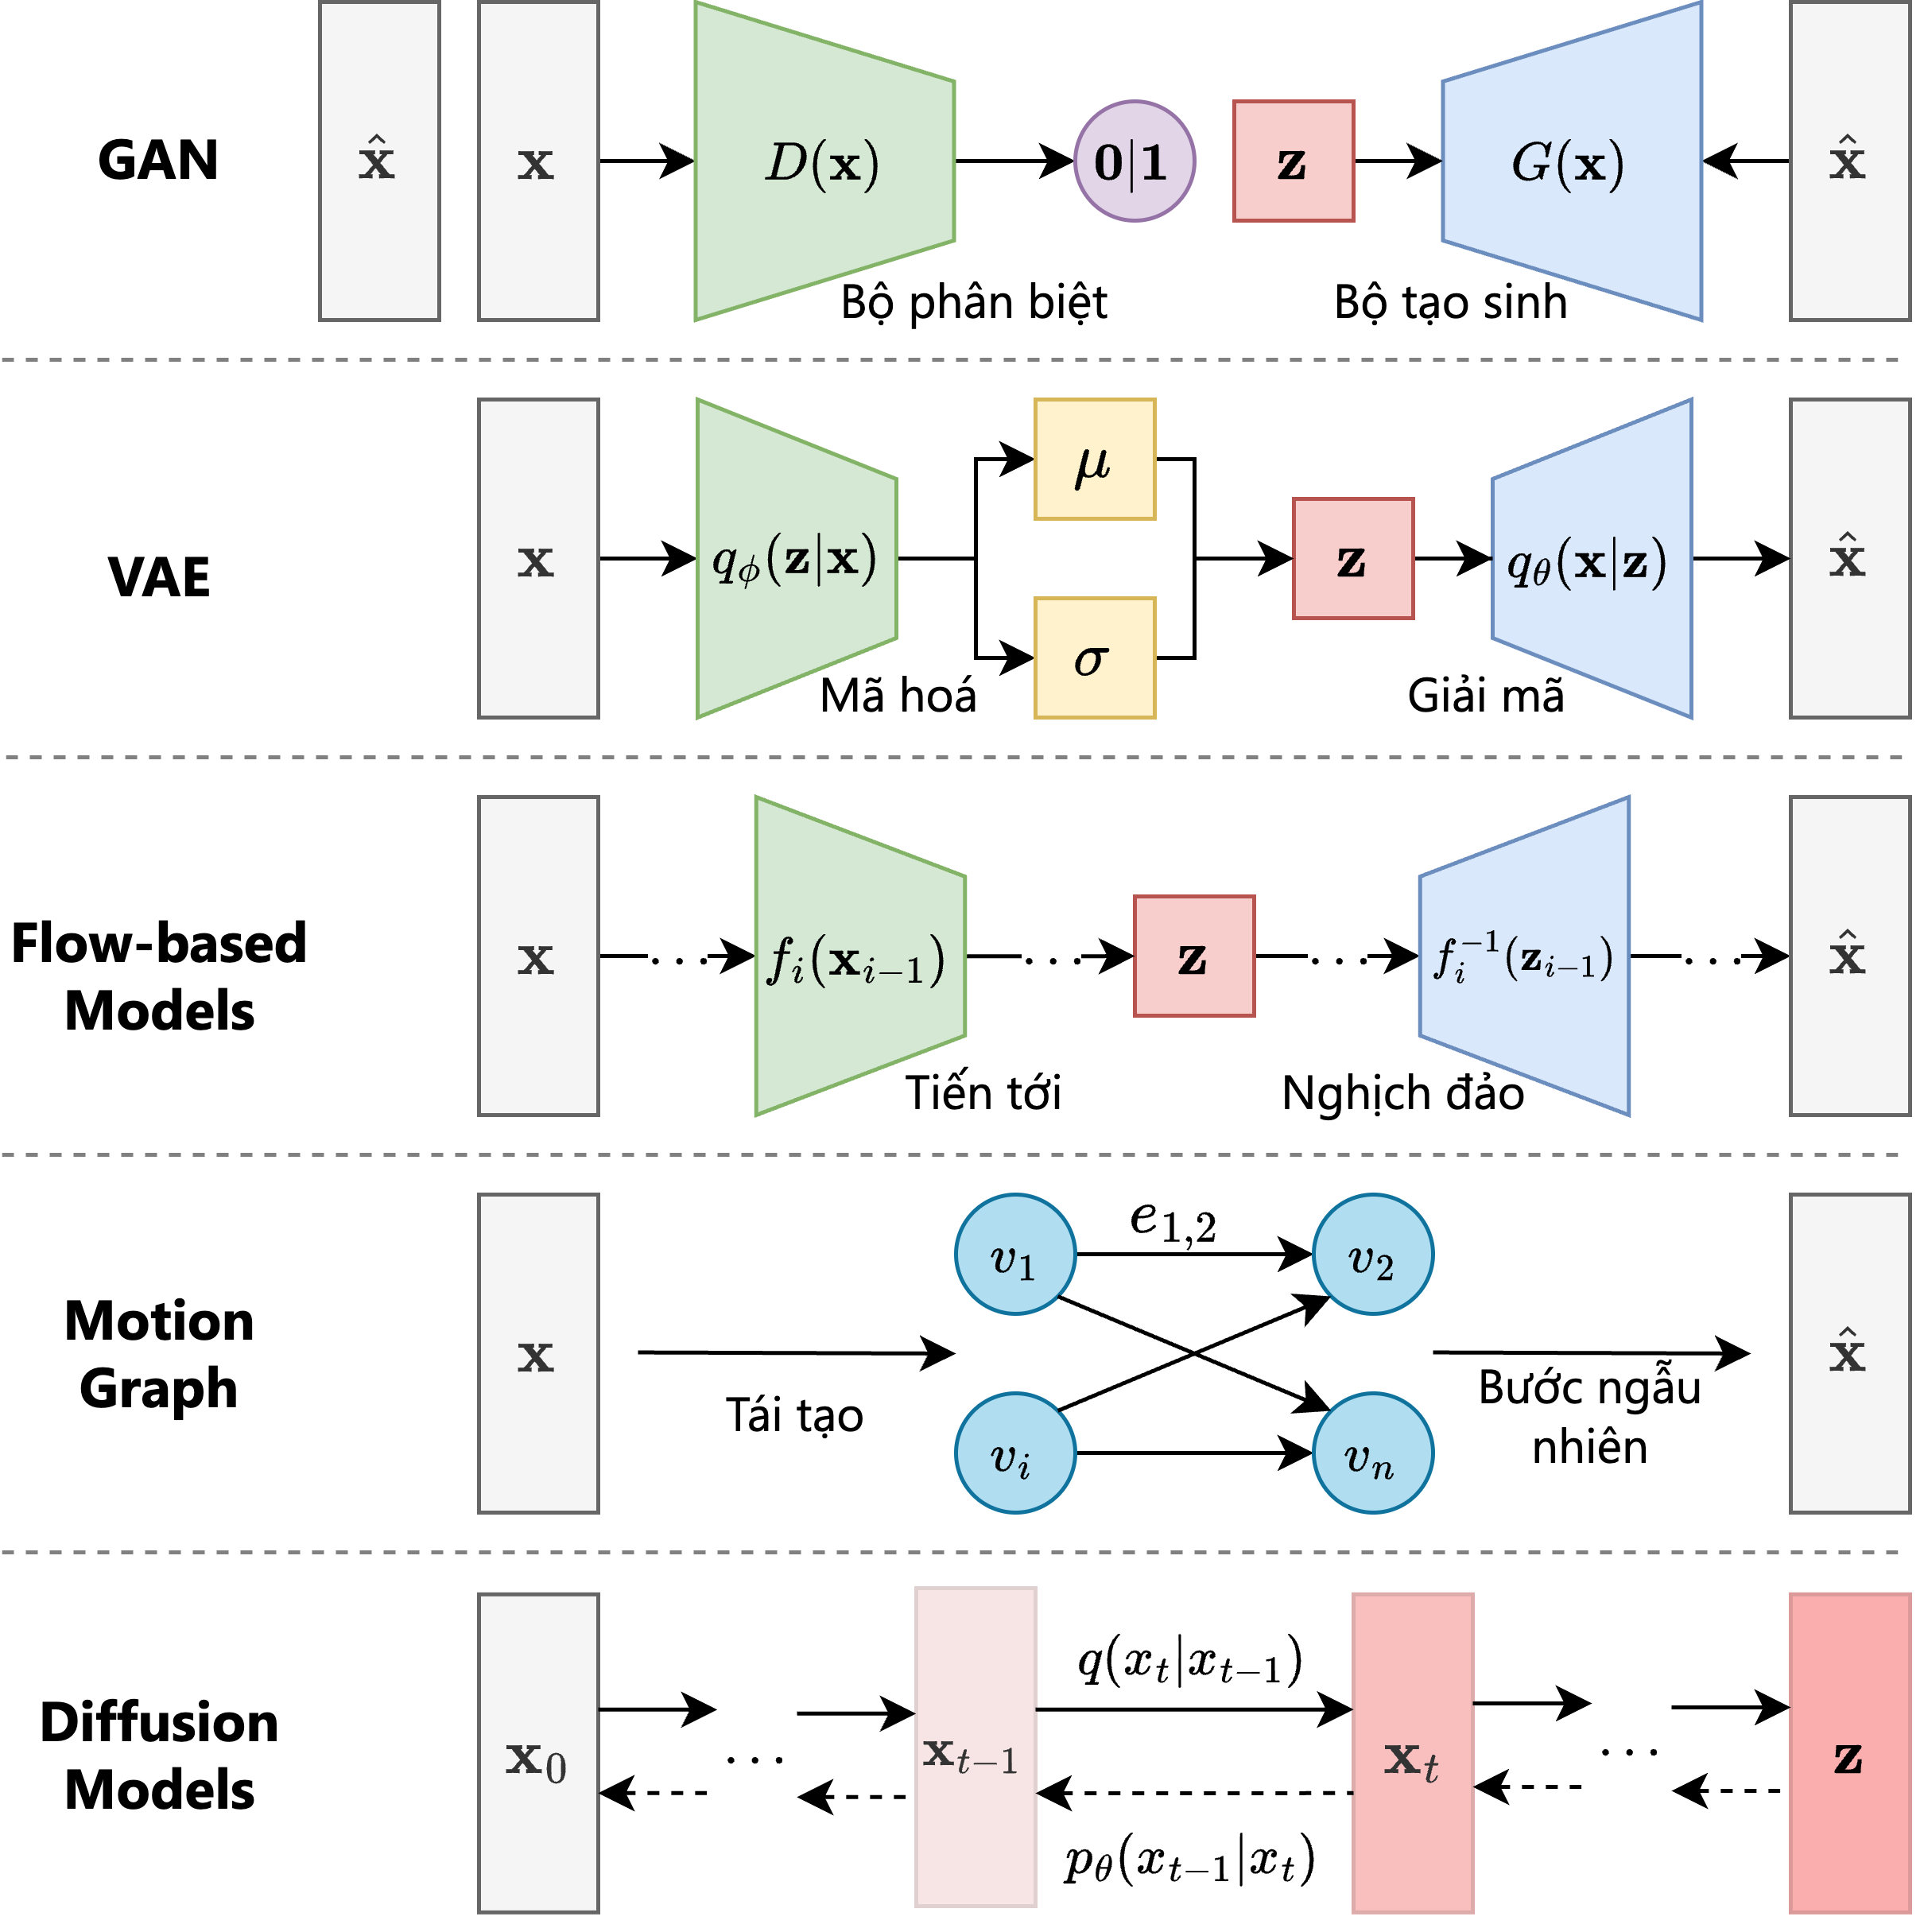
\includegraphics[width=\linewidth]{figures/GeneralOverview}
%	\caption{Overview of different generative models.}
%	\label{fig:GeneralOverview}
%\end{figure}

Deep learning-based gesture generation methods can be divided into two main groups: likelihood-based models and implicit generative models \cite{song2021score}.


\textbf{Likelihood-Based Models}

These models work by maximizing the likelihood of observed data given model parameters $\theta$. The objective is to find the optimal parameters $\theta'$ by modeling the probability $p(\mathbf{x})$ of the data, where $\mathbf{x}$ represents the gesture sequence.


\textbf{Methods}: The application of deep learning to gesture generation has evolved alongside the development of deep learning models, including RNNs, LSTMs, and Transformers. Representative likelihood-based methods include:

\begin{itemize}
	\item \textit{Gesticulator} \cite{kucherenko2020gesticulator}, which uses a Multilayer Perceptron (MLP) to encode text and audio features, with BERT-derived vectors used as text features.
	
	\item \textit{HA2G} \cite{liu2022learning} builds a hierarchical Transformer-based model to learn multi-level correlations between speech and gestures, from local to global features.
	
	\item \textit{Gesture Generation from Trimodal Context} \cite{yoon2020speech} uses an RNN architecture and treats gesture generation as a translation task in natural language processing.
	
	\item \textit{DNN} \cite{chiu2015predicting} combines LSTM and GRU to build a classifier neural network that selects appropriate gesture units based on speech input.
	
	\item \textit{Cascaded Motion Network (CaMN)} \cite{liu2022beat} introduces the BEAT dataset and a waterfall-like model. Speaker information, emotion labels, text, speech, and gesture features are processed through layers to extract latent vectors. In the fusion stage, CaMN combines features sequentially: speaker and emotion features are merged first, followed by integration with latent vectors of text, speech, and gestures.
	
	\item \textbf{Motion Graph}: In \textit{Gesturemaster} \cite{zhou2022gesturemaster}, a semantic graph is constructed where words in a sentence are connected based on semantic relationships. The model then selects the most relevant nodes and edges in the graph to represent gestures.
\end{itemize}


%\vfill
%\begin{figure*}[htbp]
%	\centering
%	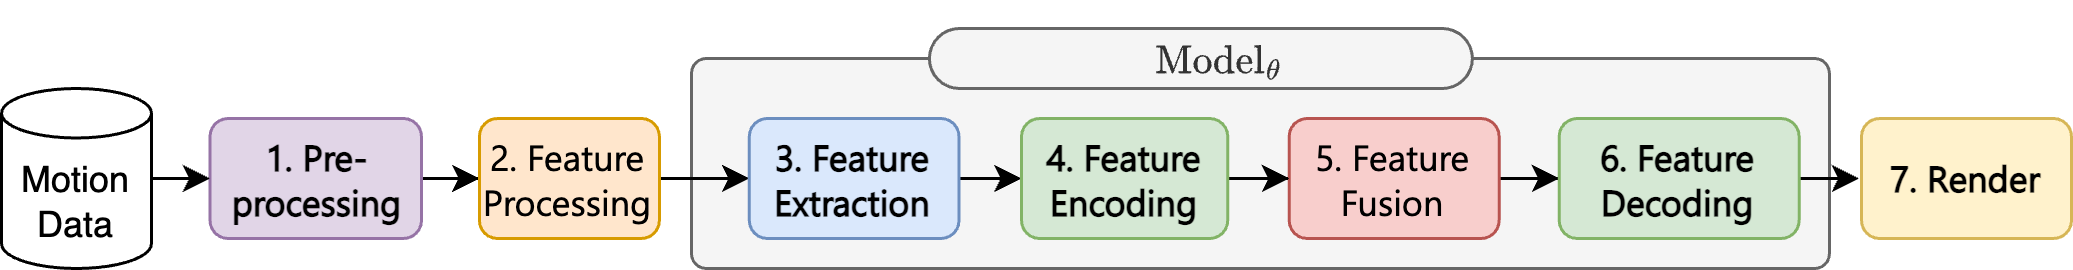
\includegraphics[width=0.9\linewidth]{figures/CommonStage.png}
%	\caption{Common stages in gesture generation models.}
%	\label{fig:CommonStage}
%\end{figure*}

\begin{figure*}[htbp]
	\centering
	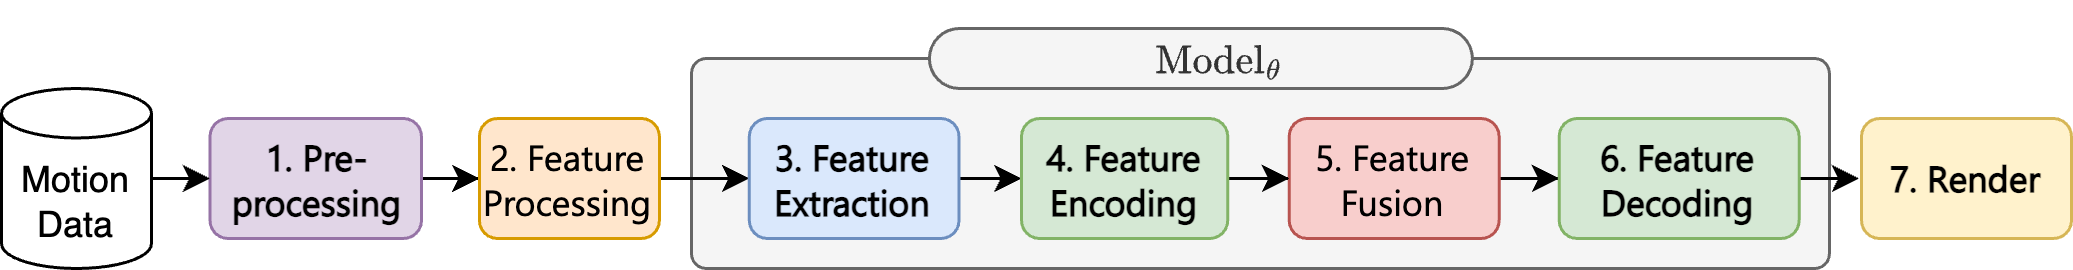
\includegraphics[width=0.9\linewidth]{figures/CommonStage.png}
%	\resizebox{\textwidth}{!}{%\begin{tikzpicture}[
%	box/.style={rounded corners, draw, fill=#1, minimum width=2cm, minimum height=1cm, align=center},
%	arrow/.style={->, >=stealth},
%	cylinder/.style={shape=cylinder, draw, minimum height=1.5cm, minimum width=0.8cm, shape aspect=2, align=center}
%	]
%	
%	% Boxes
%	\node[box=#e1d5e7, fill=#e1d5e7, draw=#9673a6] (preprocess) at (2,-3) {\textbf{1. Pre-processing}};
%	\node[box=#ffe6cc, fill=#ffe6cc, draw=#d79b00, right=1cm of preprocess] (featureproc) {2. Feature Processing};
%	\node[box=#dae8fc, fill=#dae8fc, draw=#6c8ebf, right=1cm of featureproc] (featureext) {\textbf{3. Feature Extraction}};
%	\node[box=#d5e8d4, fill=#d5e8d4, draw=#82b366, right=1cm of featureext] (featureenc) {\textbf{4. Feature Encoding}};
%	\node[box=#f8cecc, fill=#f8cecc, draw=#b85450, right=1cm of featureenc] (featurefus) {5. Feature Fusion};
%	\node[box=#d5e8d4, fill=#d5e8d4, draw=#82b366, right=1cm of featurefus] (featuredec) {\textbf{6. Feature Decoding}};
%	\node[box=#fff2cc, fill=#fff2cc, draw=#d6b656, right=1cm of featuredec] (render) {\textbf{7. Render}};
%	
%	% Cylinder
%	\node[cylinder, below left=0.5cm and 1cm of preprocess] (motiondata) {Motion\\Data};
%	
%	% Model box
%	\node[rounded corners, draw, fill=#f5f5f5, minimum width=6cm, minimum height=0.7cm, above=0.5cm of featureext] (model) {$\text{Model}_\theta$};
%	
%	% Arrows
%	\draw[arrow] (motiondata.east) -- (preprocess.west);
%	\draw[arrow] (preprocess) -- (featureproc);
%	\draw[arrow] (featureproc) -- (featureext);
%	\draw[arrow] (featureext) -- (featureenc);
%	\draw[arrow] (featureenc) -- (featurefus);
%	\draw[arrow] (featurefus) -- (featuredec);
%	\draw[arrow] (featuredec) -- (render);
%	
%\end{tikzpicture}

\begin{tikzpicture}[
	box/.style={rounded corners, draw, fill=#1, minimum width=2cm, minimum height=1cm, text width = 30mm,align=center},
	arrow/.style={->, >=stealth},
	cylinder/.style={shape=cylinder, draw, minimum height=1.5cm, minimum width=0.8cm, shape aspect=2, align=center}
	]
	
	% Boxes
	\node[draw=preprocessdraw, fill=preprocessfill, box=preprocessfill] (preprocess) at (2,-3) {\textbf{1. Pre-processing}};
	\node[draw=featureprocdraw, fill=featureprocfill, box=featureprocfill, right=0.5cm of preprocess] (featureproc) {2. Feature Processing};
	\node[draw=featureextdraw, fill=featureextfill, box=featureextfill, right=0.5cm of featureproc] (featureext) {\textbf{3. Feature Extraction}};
	\node[draw=featureencdraw, fill=featureencfill, box=featureencfill, right=0.5cm of featureext] (featureenc) {\textbf{4. Feature Encoding}};
	\node[draw=featurefusdraw, fill=featurefusfill, box=featurefusfill, right=0.5cm of featureenc] (featurefus) {5. Feature Fusion};
	\node[draw=featuredecdraw, fill=featuredecfill, box=featuredecfill, right=0.5cm of featurefus] (featuredec) {\textbf{6. Feature Decoding}};
	\node[draw=renderdraw, fill=renderfill, box=renderfill, right=0.5cm of featuredec] (render) {\textbf{7. Render}};
	
	% Cylinder
	\node[cylinder, left=0.5cm and 0.5cm of preprocess] (motiondata) {\text{Motion Data}};
	
	% Model box
	\node[rounded corners, draw, fill=modelfill, minimum width=6cm, minimum height=0.7cm, above=0.5cm of featureext] (model) {$\text{Model}_\theta$};
	
	% Arrows
	\draw[arrow] (motiondata.east) -- (preprocess.west);
	\draw[arrow] (preprocess) -- (featureproc);
	\draw[arrow] (featureproc) -- (featureext);
	\draw[arrow] (featureext) -- (featureenc);
	\draw[arrow] (featureenc) -- (featurefus);
	\draw[arrow] (featurefus) -- (featuredec);
	\draw[arrow] (featuredec) -- (render);
	
\end{tikzpicture}}
	\caption{Common stages in gesture generation models.}
	\label{fig:CommonStage}
\end{figure*}

\textbf{Implicit Generative Models}
\label{sec:ImplicitGenerativeModels}

Implicit generative models learn the data distribution without explicitly modeling the probability density function $p(\bx)$. Instead of directly computing $p(\bx)$, the model learns a mapping $G_{\theta}: \mathcal{Z} \to \mathcal{X}$ by matching the distributions between real and generated data $\mathbf{x} = G_\theta(\mathbf{z}), \quad \mathbf{z} \sim p_z(\mathbf{z})$. Here, $\mathcal{Z}$ denotes the input noise space, typically with a simple distribution \(p_{z}\) (e.g., Gaussian, Uniform), and \(\mathcal{X}\) is the space of real data, which in this case is gesture sequences \(\mathbf{x}\).

In gesture generation, to incorporate conditions such as speech or text labels, implicit generative models often introduce a condition $\mathbf{c}$ representing the context of the task, resulting in the conditional generation: $\mathbf{x} = G_\theta(\mathbf{z}, \mathbf{c})$. This context may include speech, text, speaker ID, style, emotion, or initial gestures.

A typical example is the generative adversarial network (GAN) and Diffusion model, where data is synthesized by transforming an initial simple distribution (e.g., Gaussian) into the target data distribution.


\textbf{Methods}: Representative implicit generative models include:

\begin{itemize}
	\item \textit{MoGlow} \cite{henter2020moglow} uses Normalizing Flows to maintain motion consistency and compatibility, while providing control via input parameters. This allows users to generate new motions or modify existing ones by adjusting control parameters.
	
	\item \textbf{GAN}: \textit{GRU-based WGAN} \cite{wu2021probabilistic} utilizes Wasserstein GAN to evaluate and improve the quality of gesture synthesis. The model focuses on optimizing the Wasserstein loss, mitigating mode collapse typically seen in traditional GANs. GRUs process speech data and convert it into usable gesture features, which are then fed into the WGAN for evaluation and refinement.
	
	\item \textbf{VAE}: \textit{FreeMo} \cite{xu2022freeform} employs a VAE to decompose gestures into pose modes and rhythmic motions. Gesture poses are randomly sampled using conditional sampling in the VAE's latent space, while rhythmic motions are generated from...
	
	\item \textbf{VQ-VAE}: \textit{Rhythmic Gesticulator} \cite{ao2022rhythmic} preprocesses speech segments based on beats, dividing speech into smaller parts and representing them as blocks with normalized dimensions. Similar to the VQ-VAE approach, normalized gesture sequences are quantized into discrete gesture lexicons. The model learns the gesture vocabulary conditioned on the previous gesture, gesture style, and speech. It then reconstructs the gesture sequence via denormalization. Unlike generative models like GANs or Diffusion, VQ-VAE focuses more on compression rather than direct generation.
	
	\item \textbf{Diffusion}: Diffusion models focus on generating new data from noisy inputs by progressively denoising toward the original data. Diffusion-based approaches will be presented in \autoref{sec:diffusionbase}.
\end{itemize}




\subsection{Common Stages in Deep Learning Approaches for Gesture Generation}
\label{sec:commonstage}

As presented in \autoref{sec:Data}, gestures consist of sequences of 3D point coordinates. For each dataset, the number of bones per frame may vary.


Deep learning approaches to gesture generation are implemented using various techniques. However, we generalize the process into the following main stages, illustrated in \autoref{fig:CommonStage}:


\begin{enumerate}
	\item \textbf{Preprocessing}: In the preprocessing stage, data such as speech segments, gesture sequences, and text are read and digitized into vectors or matrices that represent raw data information. Depending on the specific learning method, the selected initial data features may vary.
	
	\item \textbf{Feature Processing}: In this stage, raw data such as speech and text are embedded into feature vectors. Different methods use different embedding models. The way gesture sequences are represented as feature vectors also varies across methods.
	
	\item \textbf{Feature Extraction}: This stage uses linear transformation layers or CNN layers to extract features from the data. Text and speech features, after being processed, may be further passed through feature extraction layers to generate representation vectors corresponding to the input modalities.
	
	\item \textbf{Feature Encoding}: In this stage, gesture, emotion, and speech vectors are encoded into a lower-dimensional latent space to facilitate learning the correlations among modalities in the feature fusion stage.
	
	\item \textbf{Feature Fusion}: In this stage, features from speech, text, gestures, and other information are combined, typically using concatenation, fully connected layers, or operations such as vector addition or subtraction in the latent space.
	
	\item \textbf{Feature Decoding}: In this stage, latent vectors are decoded or upsampled back to their original dimensionality.
	
	\item \textbf{Rendering}: Once the output vectors are restored to their original size, they are converted back into BVH files and rendered using software such as Blender or Unity to visualize character motion.
\end{enumerate}





\subsection{Diffusion-based Model for Gesture Generation}
\label{sec:diffusionbase}




\begin{itemize}
	\item \textit{MotionDiffuse} \cite{zhang2022motiondiffuse} employs a conditional Diffusion model, with conditions based solely on text, excluding audio. Additionally, the model predicts noise rather than directly predicting the original gesture sequence. MotionDiffuse utilizes Self-Attention and Cross-Attention layers to model the correlation between textual features and gesture features during \textit{Stage 5. Feature Fusion} (\autoref{fig:CommonStage}).
	
	\item \textit{Flame} \cite{kim2023flame} applies a Diffusion model with a Transformer-based architecture. In \textit{Stage 2. Feature Processing} (\autoref{fig:CommonStage}), it uses the pre-trained RoBERTa model to embed the text into textual feature vectors, which serve as the conditioning input. During \textit{Stage 5. Feature Fusion} (\autoref{fig:CommonStage}), the text is used as the $\texttt{CLS}$ token prepended to the gesture sequence before passing through the Transformer Decoder. Similar to other methods, the model predicts the added noise rather than the original gesture sequence.
	
	\item \textit{DiffWave} \cite{kong2020diffwave} is a noise-predicting Diffusion model in which the time steps pass through multiple Fully Connected layers and a Swish activation function before feature fusion. It uses a dilated convolutional architecture inherited from WaveNet. DiffWave enables better representation of speech, improving the effectiveness of conditioning for the Diffusion model.
	
	\item \textit{Listen, Denoise, Action} \cite{alexanderson2022listen} builds upon DiffWave \cite{kong2020diffwave}, replacing the dilated convolution layers with a Transformer, and integrating Conformer modules to enhance model performance.
	
	\item \textit{DiffSHEG} \cite{chen2024diffsheg} employs a Diffusion model; in \textit{Stage 2. Feature Processing}, it uses HuBERT to encode the audio signal. The model treats facial expressions as a signal for gesture generation and achieves real-time fusion of both facial expressions and gestures.
	
	\item \textit{GestureDiffuCLIP} \cite{ao2023gesturediffuclip} uses a Diffusion model conditioned on text, leveraging Contrastive Learning with CLIP to integrate text features and control gesture styles. Similar to other prompt-based approaches such as StableDiffusion or Midjourney, it treats text as prompts to learn gestures from descriptive sentences.
	
	\item \textit{Freetalker} \cite{yang2024freetalker} trains a Diffusion model on multiple datasets to generate speaker-specific gestures conditioned on speech and text. Unlike Transformer-based methods, Freetalker employs an Attention-based Network to model the correlation between textual, auditory, and gesture features during \textit{Stage 5. Feature Fusion} (\autoref{fig:CommonStage}).
\end{itemize}

\begin{figure}[htbp]
	\centering
	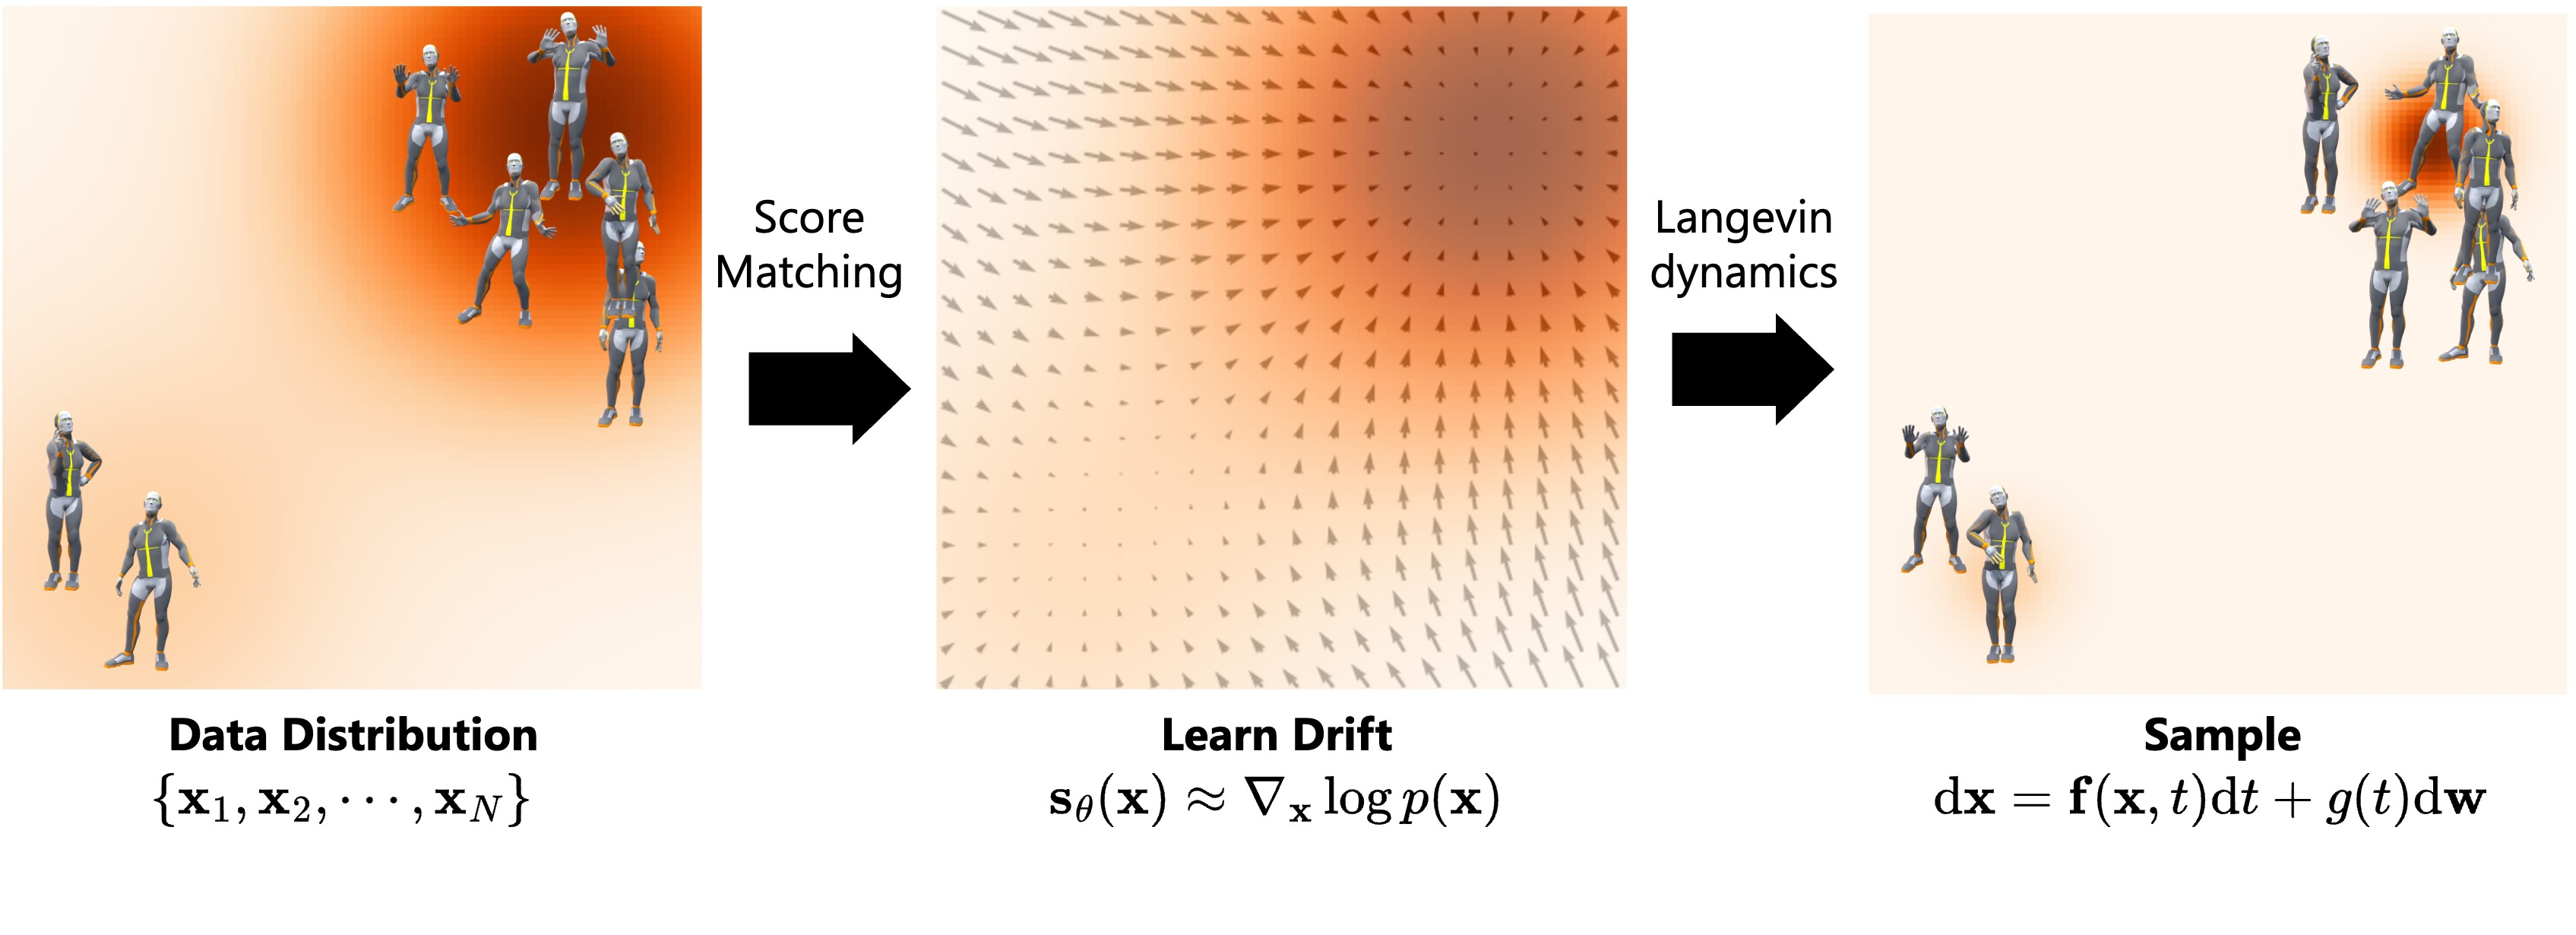
\includegraphics[width=\linewidth]{figures/ScoreMatching.jpg}
	\caption{Illustration of the diffusion drift term in gesture generation. The figure demonstrates how the learned drift guides the reverse diffusion process to synthesize temporally coherent and semantically relevant gestures from noise.}
	\label{fig:ScoreMatching}
\end{figure}

\vspace{-0.2cm}
\subsubsection{Selected Diffusion-based Methods}


\begin{itemize}
	\item \textit{MDM} \cite{tevet2022human} applies conditional Diffusion to gesture generation, using CLIP (Contrastive Language–Image Pre-training) embeddings of descriptive text as conditions. MDM adopts a Transformer-based architecture to reconstruct original gesture data. Like other text-based Diffusion approaches, in \textit{Stage 3. Feature Extraction} (\autoref{fig:CommonStage}), the input text is randomly masked to hide certain segments, enabling the model to learn the importance of each part for various gestures. 
	
	In \textit{Stage 5. Feature Fusion} (\autoref{fig:CommonStage}), the text is prepended as a $\texttt{[CLS]}$ token to the gesture sequence before passing through the Transformer Encoder, where self-attention models the relationship between the text and each gesture frame. MDM predicts the original gesture data rather than noise.
	
	\item \textbf{DiffuseStyleGesture} \cite{yang2023diffusestylegesture} extends \textit{MDM} \cite{tevet2022human} by incorporating audio, initial gestures, and style as conditioning inputs. In \textit{Stage 1. Preprocessing} (\autoref{fig:CommonStage}), the model processes coordinate vectors to obtain feature vectors of dimension $D=1141$ per frame. In \textit{Stage 2. Feature Processing} (\autoref{fig:CommonStage}), DiffuseStyleGesture uses WavLM for audio embedding. In \textit{Stage 5. Feature Fusion} (\autoref{fig:CommonStage}), it improves upon MDM by applying Cross-Local Attention prior to the Transformer Encoder.
\end{itemize}
%
%\subsubsection{Comparison of Gesture Generation Methods}
%
%
%\begin{table*}[t]
%	\small
%	\centering
%	\renewcommand{\arraystretch}{1.5}
%	\resizebox{\textwidth}{!}{
%		\begin{tabular}{|p{0.2\textwidth}|p{0.35\textwidth}|p{0.35\textwidth}|p{0.2\textwidth}|}
%			\hline
%			\textbf{Representative Method} & \textbf{Advantages} & \textbf{Disadvantages} & \textbf{Method Type} \\ \hline
%			Robot behavior toolkit \cite{huang2012robot} & 
%			- Easy to understand and implement. \newline 
%			- Highly interpretable and controllable. \newline
%			- Effective for simple cases or small datasets. & 
%			- Does not generalize well to complex data. \newline 
%			- Labor-intensive rule construction. & 
%			Rule-based model \\ \hline
%			MLP \cite{kucherenko2020gesticulator}, RNN \cite{bhattacharya2021speech2affectivegestures}, \cite{liu2022learning}, \cite{hasegawa2018evaluation}, \cite{yoon2020speech}, CNN \cite{habibie2021learning}, Transformer \cite{bhattacharya2021text2gestures}  & 
%			- Able to estimate data probability density. \newline 
%			- Scalable and learns well from large datasets. & 
%			- Sensitive to noise. \newline 
%			- Performs poorly on low-frequency data. \newline
%			- Low diversity in generation. & 
%			Likelihood-based model \\ \hline
%			\textbf{DiffusionStyle-Gesture} \cite{yang2023diffusestylegesture}, MDM \cite{tevet2022human}, Motiondiffuse \cite{zhang2022motiondiffuse} &
%			- Generates high-quality data. \newline 
%			- Flexible and diverse outputs. \newline
%			- Covers low-density regions of data space. & 
%			- Requires complex configuration for optimal performance. \newline 
%			- Random noise leads to different outputs each time. \newline 
%			- Slow sampling process. & 
%			Implicit generative model \\ \hline
%		\end{tabular}
%	}
%	\caption{Comparison of advantages and disadvantages of different methods}
%	\label{table:CompareMethod}
%\end{table*}


